\documentclass[11pt,a4paper]{article}
\usepackage[margin=2.4cm]{geometry}
\usepackage{amsmath,amssymb,bm,graphicx,booktabs,xcolor}
\usepackage[numbers,sort&compress]{natbib}
\usepackage[colorlinks,citecolor=blue!60!black,linkcolor=blue!60!black,urlcolor=blue!60!black]{hyperref}
\graphicspath{{figures/}{../figures/}}
\newcommand{\todo}[1]{\textcolor{red}{[TODO: #1]}}
\newcommand{\Mpl}{M_{\rm pl}}
\newcommand{\aeff}{\alpha_{\rm eff}}
\newcommand{\et}{\tilde\epsilon}

\title{How much of the dark-energy potential can late-time data see?\\[2pt]
\large Differentiable forward modelling of $V(\phi)$ in quadratic gravity}
\author{\todo{authors (supervisor too?), affiliation, e-mail}}
\date{\todo{date}}

\begin{document}
\maketitle

\begin{abstract}
Recent model-independent reconstructions of the quintessence potential differentiate a regressed expansion history, which amplifies noise and can return a negative kinetic energy. We return to direct reconstruction, in which $V(\phi)$ sits inside the field equations and distances are fitted directly, and make it free-form: $V$ is a small neural network trained by differentiating through the ODE solver. Gravity is allowed a quadratic deformation $R+\alpha R^2+\beta R_{\mu\nu}R^{\mu\nu}$, of which only $\alpha+\beta/3$ is visible on FLRW backgrounds. On the branch connected to general relativity it adds $\tfrac{27}{2}\epsilon\,\Omega_m^2a^{-6}$ to $H^2/H_0^2$. Using 15 cosmic chronometers, DESI DR2 BAO and Pantheon+ (1608 points), an exact Fisher analysis in function space shows that, because the field moves by only $0.25\,\Mpl$, the data are sensitive to two numbers about $\ln V$: its height and its slope. A curvature would have to exceed $|V''/V|\approx9\,\Mpl^{-2}$ to be seen at $1\sigma$. An exponential potential improves the fit over $\Lambda$CDM by $\Delta\chi^2=-4.9$ for one parameter ($w_0=-0.90\pm0.05$); a 321-parameter network improves it by only a further $0.4$. On 50 mock data sets at each of two truths, the bootstrap ensemble's 68\% and 95\% intervals are about as well calibrated as MCMC posteriors, but its median overstates the drop in $V$ by $0.5$--$1\sigma$, most when the field barely rolls. With a cosmological constant we find $\epsilon<4.1\times10^{-4}$ (95\%) at first order in the order reduction. The reduced equation is a divergent series: at this value its second-order term is already 28\% of the first at $z=2.33$, and at second order the data give no bound independent of the prior, so the limit holds only to order of magnitude. The first-order bound weakens twenty-fold and becomes degenerate with $\omega_m$ once $V$ is free. No model raises $H_0$. Features in reconstructed potentials beyond a slope are not supported by current background data.
\end{abstract}

%=====================================================================
\section{Introduction}
%=====================================================================
The DESI DR2 baryon-acoustic-oscillation (BAO) measurements~\cite{2503.14738}, combined with supernovae, have renewed interest in dynamical dark energy. In particular, they have revived interest in thawing quintessence, a scalar field held by Hubble friction until recently.
The natural theoretical target is the potential $V(\phi)$, and there are two ways to reconstruct it.
\begin{itemize}
\item \emph{Direct reconstruction} places a parametrised $V$ inside the field equations and fits the data with the resulting solutions. Examples are Taylor and Pad\'e expansions with the order chosen by an information criterion~\cite{astro-ph_0506696,astro-ph_0610812}, a binned potential~\cite{astro-ph_0611093}, polynomial potentials evolved with flow equations~\cite{astro-ph_0610427}, and an effective-field-theory reconstruction in time from which $V(\Delta\phi)$ follows~\cite{2101.04666}. Recent fits of linear, quadratic and exponential potentials to DESI data are of this kind~\cite{2505.10662,2405.17396,2404.14341}.
\item \emph{Regression and inversion} regresses $H(z)$ with a Gaussian process~\cite{2203.06767,2112.09722,2305.04752,2603.21125,2604.04056,2608.24433,2411.00051} or a neural network~\cite{2305.15500}, then inverts the Friedmann and Klein--Gordon equations. The inversion needs $H'$, and for the slope of $V$ also $H''$. Derivatives of a regressed curve are dominated by the kernel or architecture, and $\dot\phi^2$, a difference of noisy terms, can come out negative~\cite{2603.21125}.
\end{itemize}
Most recent ``model-independent'' work, including the machine-learning reconstructions, follows the second route. Direct reconstructions have used low-order expansions or bins in $\phi$, or splines in time.

Machine learning has entered background cosmology in other ways too:
\begin{itemize}
\item as a fast replacement for the ODE solver~\cite{2205.02945,2311.15955,2506.05674};
\item as a physics-informed regressor of $H(z)$ or $w(z)$~\cite{2403.13899,2605.30139,2606.17614};
\item through symbolic regression~\cite{2211.11461,2502.10506,2606.17951};
\item through simulation-based inference~\cite{2606.16248,2412.12323}.
\end{itemize}
Differentiable likelihood codes exist for fixed parametric backgrounds~\cite{2302.05163,2606.28175,2609.28458}.

We follow the direct route with a free-form parametrisation, using the construction known in scientific machine learning as a universal differential equation~\cite{2001.04385,1806.07366}. The ODE is kept exact, $V$ inside it is a neural network, and the data are fitted by differentiating through the solver. Every reconstruction is then a solution of the field equations, so $\dot\phi^2\ge0$ by construction.

The exact Jacobian of the data vector with respect to a function-space basis for $\ln V$ comes almost for free. It answers a question older than the method: how many features of $V$ do the data measure? Counting constrained modes is standard for the dark-energy equation of state~\cite{astro-ph_0207517,1004.0236} and for the inflaton potential~\cite{astro-ph_0505158}. Park et al.\ count the quintessence parameters constrained by CMB, large-scale-structure and supernova data~\cite{2101.04666}. Here we do it for $\ln V(\phi)$ with background data in the DESI DR2 era.

We also let gravity deviate from general relativity (GR) by the quadratic terms $\alpha R^2+\beta R_{\mu\nu}R^{\mu\nu}$, a one-parameter deformation that competes with the shape of $V$. Recent analyses constrain an $R_{\mu\nu}R^{\mu\nu}$ correction with a cosmological constant~\cite{2607.22126}, and $f(R)$ models in which the modified gravity itself drives the acceleration~\cite{2305.06392,2112.00822,2609.21912,2511.06924}; in neither case is a dark-energy potential varied at the same time. Here we quantify the degeneracy between the two. The quadratic sector is a controlled test case, not a viability claim. Laboratory and gravitational-wave bounds on $R^2$~\cite{hep-ph_0611184,1104.0819,2611.06902} are tens of orders of magnitude below what cosmological backgrounds can reach (Sec.~\ref{sec:bounds}).

\paragraph{Contributions.}
\begin{enumerate}
\item \emph{What current background data measure about $V(\phi)$.} From an exact function-space Fisher matrix, chronometers, DESI DR2 BAO and Pantheon+ are sensitive to the height and slope of $\ln V$ only, because the field moves by $0.25\,\Mpl$. A 321-parameter potential improves $\chi^2$ by only 0.4 over an exponential. This agrees with the finding that a quadratic term improves a linear-potential fit to DES-SN5YR and DESI DR2 by $\Delta\chi^2<1$~\cite{2505.10662}, and quantifies it.
\item \emph{Calibrated uncertainties.} A coverage test, on 50 mocks at each of two truths, of the bootstrap ensemble against MCMC posteriors.
\item \emph{Quadratic gravity as a competing deformation.} The order-reduced correction to all orders, which is a divergent series that limits any $\epsilon$ bound to order of magnitude, a test against the full third-order equation, and the degeneracy between $\epsilon$ and the shape of $V$.
\item \emph{A free-form direct reconstruction:} a neural $V(\phi)$ inside a differentiable solver. We are not aware of a previous late-time quintessence reconstruction with a neural potential inside the solver. \todo{rerun \texttt{paper/citation\_trail.py} before submission.}
\end{enumerate}

%=====================================================================
\section{Theory}\label{sec:theory}
%=====================================================================
\subsection{Action and field equations}
We consider
\begin{equation}
S=\int d^4x\sqrt{-g}\left[\frac{R+\alpha R^2+\beta R_{\mu\nu}R^{\mu\nu}}{2\kappa^2}-\tfrac12(\partial\phi)^2-V(\phi)\right]+S_m ,
\label{eq:action}
\end{equation}
with signature $(-,+,+,+)$, $c=1$ and $\kappa^2=8\pi G=\Mpl^{-2}$. Varying with respect to the metric gives
\begin{equation}
G_{\mu\nu}+\alpha E^{(1)}_{\mu\nu}+\beta E^{(2)}_{\mu\nu}=\kappa^2\left(T^{(m)}_{\mu\nu}+T^{(\phi)}_{\mu\nu}\right),\qquad \Box\phi-V_{,\phi}=0,
\end{equation}
with $E^{(1,2)}_{\mu\nu}$ given in Appendix~\ref{app:variation}. The trace,
\begin{equation}
-R+(6\alpha+2\beta)\Box R=\kappa^2T,
\end{equation}
shows an extra scalar mode (the scalaron) with mass $m_0^2=1/(6\alpha+2\beta)$.
The $R_{\mu\nu}R^{\mu\nu}$ term also carries a massive spin-2 ghost with $m_2^2=-1/\beta$~\cite{Stelle1977}. The ghost does not appear on FLRW backgrounds, but it limits the full theory to an effective field theory.
\subsection{Only $\alpha+\beta/3$ is observable on FLRW}
In four dimensions the Gauss--Bonnet combination $\mathcal G=R^2-4R_{\mu\nu}R^{\mu\nu}+R_{\mu\nu\rho\sigma}R^{\mu\nu\rho\sigma}$ is a total derivative. The Weyl-squared invariant $C^2=R_{\mu\nu\rho\sigma}R^{\mu\nu\rho\sigma}-2R_{\mu\nu}R^{\mu\nu}+\tfrac13R^2$ is quadratic in a tensor that vanishes on FLRW, so its variation vanishes there.
Hence $\mathcal G-C^2=\tfrac23R^2-2R_{\mu\nu}R^{\mu\nu}$ does not contribute to FLRW equations, and
\begin{equation}
\alpha R^2+\beta R_{\mu\nu}R^{\mu\nu}\;\simeq\;\left(\alpha+\tfrac{\beta}{3}\right)R^2\equiv\aeff R^2 .
\end{equation}
This follows from the identity $R_{\mu\nu}R^{\mu\nu}=\tfrac13R^2+\tfrac12(C_{\mu\nu\rho\sigma}C^{\mu\nu\rho\sigma}-\mathcal{G})$, where $\mathcal{G}$ is the Gauss--Bonnet invariant~\cite{1002.4928}. In four dimensions $\mathcal{G}$ does not contribute to the field equations, and the Weyl term contributes only through the Bach tensor, which vanishes on the conformally flat FLRW metric. We confirmed it symbolically: substituting a lapse-dependent FLRW metric into each invariant and varying, the $R_{\mu\nu}R^{\mu\nu}$ term gives exactly one third of the $R^2$ term. Expansion data therefore cannot separate $\alpha$ from $\beta$; separate posteriors would reflect priors only.

\subsection{Friedmann and scalar equations}
With $H=\dot a/a$ and $R=6(2H^2+\dot H)$, the $(00)$ equation is
\begin{equation}
H^2+6\aeff\left(2H\ddot H-\dot H^2+6H^2\dot H\right)=\frac{\kappa^2}{3}\left(\rho_m+\rho_r+\tfrac12\dot\phi^2+V\right),
\label{eq:friedmann}
\end{equation}
together with $\ddot\phi+3H\dot\phi+V_{,\phi}=0$ and the usual continuity equations. Equation~\eqref{eq:friedmann} is third order in $a(t)$. The extra initial condition is the scalaron amplitude.

\subsection{Order reduction and its validity}\label{sec:reduction}
For $m_0\gg H$ the scalaron oscillations are stiff and absent unless put in by hand. The solution continuous with GR as $\aeff\to0$ is obtained by evaluating the bracket in Eq.~\eqref{eq:friedmann} with the GR relations $\dot H=-\tfrac{\kappa^2}{2}(\rho+p)$ and $\ddot H=-\tfrac{\kappa^2}{2}(\dot\rho+\dot p)$~\cite{Simon1990,gr-qc_9211002}. For matter plus $\Lambda$ this gives
\begin{equation}
\frac{H^2}{H_0^2}=\Omega_ma^{-3}+\Omega_\Lambda+\frac{27}{2}\,\epsilon\,\Omega_m^2a^{-6},\qquad \epsilon\equiv\frac{\aeff H_0^2}{c^2}.
\label{eq:reduced}
\end{equation}
The correction acts like a stiff fluid. It vanishes in the radiation era, where $R=0$.
\begin{itemize}
\item \emph{Validity.} The reduction requires $54\,\epsilon\,\Omega_m(1+z)^3\ll1$, the ratio of the second- to the first-order term (below). For $\epsilon=10^{-4}$ this fails beyond $z\approx7$.
  \begin{itemize}
  \item A value of $\epsilon$ visible at $z<2.4$ therefore cannot be extrapolated to recombination.
  \item Conversely, a standard matter era back to $z\sim10^3$ requires $\epsilon\lesssim10^{-10}$.
  \end{itemize}
  We define the model for $z\le4$ and treat the sound horizon $r_d$ as external, as in Ref.~\cite{2607.22126}.
\item \emph{Stability.} A non-tachyonic scalaron requires $\aeff>0$~\cite{astro-ph_0307285}, so we impose $\epsilon\ge0$.
\item \emph{Accuracy.} Section~\ref{sec:validation} tests Eq.~\eqref{eq:reduced} against a direct solve of Eq.~\eqref{eq:friedmann}. Near the bounds we obtain, the two differ by as much as the correction itself.
\item \emph{Higher orders.} Writing $H^2=\sum_k\epsilon^kf_k(a)$ in Eq.~\eqref{eq:friedmann}, the bracket acts as a bilinear form that maps powers of $a$ to powers of $a$, so each $f_k$ follows algebraically. For matter and $\Lambda$ the second order adds $-729\,\epsilon^2\Omega_m^3a^{-9}-1458\,\epsilon^2\Omega_m^2\Omega_\Lambda a^{-6}$ to Eq.~\eqref{eq:reduced}. The coefficients then grow factorially, as expected when the small parameter multiplies the highest derivative, so the series is asymptotic. At $\epsilon=4.1\times10^{-4}$ and $z=2.33$ the second-order term is 28\% of the first and the third is as large as the second. The branch connected to GR is therefore defined only up to about the second-order term. Truncating at second order does not help. The correction then grows with $\epsilon$ only up to $\epsilon\approx7\times10^{-4}$ at $z=2.33$ and falls beyond, so the likelihood is not monotonic in $\epsilon$. The second-order posterior keeps 11\% of its peak density at the prior edge ($\et=2\times10^{-3}$) and gives no bound independent of the prior.
\end{itemize}

\subsection{Local and gravitational-wave bounds}\label{sec:bounds}
Late-time data are sensitive to $\epsilon\sim10^{-4}$, i.e.\ $\aeff\sim10^{48}\,{\rm m^2}$. These bounds are far tighter:
\begin{itemize}
\item Torsion-balance tests~\cite{hep-ph_0611184}, as quoted in Ref.~\cite{1104.0819}, give $|a_2|<2\times10^{-9}\,{\rm m^2}$ for $f=R+a_2R^2/2$.
\item Binary-neutron-star waveforms give $a\lesssim6.2\times10^{6}\,{\rm m^2}$~\cite{2611.06902}.
\end{itemize}
$R^2$ has no screening mechanism, so these bounds apply directly. The cosmological fits below are therefore a consistency exercise and a test of degeneracies, not evidence for or against quadratic gravity.

\subsection{Equations as integrated}
We integrate in $N=\ln a$ from $z_i=4$ to $z=0$, using these dimensionless variables:
\begin{itemize}
\item $\tilde H=H/(100\,{\rm km\,s^{-1}\,Mpc^{-1}})$;
\item $\phi$ in units of $\Mpl$, and $y=\dot\phi$;
\item $u=\kappa^2V/(3\cdot100^2)$;
\item $\omega_m=\Omega_mh^2$, $\omega_r=4.184\times10^{-5}$, and $\et=\epsilon/h^2$.
\end{itemize}
The system is
\begin{align}
\tilde H^2&=\omega_me^{-3N}+\omega_re^{-4N}+\tfrac{y^2}{6}+u(\phi)-6\et B,\quad B=2\tilde H_0\ddot{\tilde H}-\dot{\tilde H}^2+6\tilde H_0^2\dot{\tilde H},\\
\frac{d\phi}{dN}&=\frac{y}{\tilde H},\qquad \frac{dy}{dN}=-3y-\frac{3u_{,\phi}}{\tilde H},\qquad \frac{dI}{dN}=\frac{e^{-N}}{\tilde H},
\end{align}
where $\tilde H_0$, $\dot{\tilde H}$ and $\ddot{\tilde H}$ in $B$ are the GR ($\et=0$) expressions. The comoving distance is $D_C(z)=(c/100)[I(0)-I(N)]$, and $h=\tilde H(0)$ is an output.

Initial conditions:
\begin{itemize}
\item $\phi_i=0$, since only differences of $\phi$ matter;
\item $y_i=-\tfrac23u_{,\phi}/\tilde H_i$, the matter-era attractor of a field held by Hubble friction.
\end{itemize}
For $u_{,\phi}=0$ and $\et=0$ the system reduces exactly to $\Lambda$CDM.

%=====================================================================
\section{Method}\label{sec:method}
%=====================================================================
\paragraph{Differentiable solver.} The system is integrated with fixed-step fourth-order Runge--Kutta (RK4) in $N$, batched over parameter sets. Distances are read off a cubic-Hermite interpolant, with $H$ taken from $dI/dN$.
\begin{itemize}
\item The numpy version (64--512 steps) is used for MCMC.
\item The PyTorch version (48 steps) is used for gradients.
\end{itemize}
Both agree on the total $\chi^2$ to $4\times10^{-5}$.

\paragraph{Neural potential.} $\ln u(\phi)$ is a $1$-$16$-$16$-$1$ tanh multilayer perceptron with 321 weights. It is trained together with $\ln\omega_m$ and $\ln r_d$ by minimising
\begin{equation}
\mathcal L=\chi^2_{\rm CC}+\chi^2_{\rm BAO}+\chi^2_{\rm SN}+\left(\frac{r_d-\bar r_d}{\sigma_{r_d}}\right)^2+\lambda_w\|\bm w\|^2 ,
\end{equation}
with weight decay $\lambda_w=10^{-3}$. Gradients come from reverse-mode automatic differentiation through the solver. Training settings:
\begin{itemize}
\item Adam with learning rate $10^{-2}$, cosine-annealed to $2\times10^{-4}$ over 1000 iterations;
\item gradient-norm clipping at 50.
\end{itemize}

\paragraph{Uncertainty: bootstrap ensemble.} We train 24 members:
\begin{itemize}
\item member 0 on the data;
\item members 1--23 on parametric bootstrap replicas, i.e.\ the data plus Gaussian noise drawn from the full covariance, with $\bar r_d$ fluctuated likewise.
\end{itemize}
Quantiles over members 1--23 define the intervals. With 23 members, the central ``68\%'' and ``95\%'' intervals contain the truth for 16 and 22 of the 24 possible ranks. Their effective levels are therefore 67\% and 92\%; the ``95\%'' interval is the full member range. For a near-linear model with Gaussian noise this approximates the posterior (randomised maximum likelihood). Here we do not assume this; we test it on mocks (Sec.~\ref{sec:coverage}).

\paragraph{Identifiability: function-space Fisher matrix.} Around a fiducial potential we write
\begin{equation}
\ln u(\phi)\;\to\;\ln u(\phi)+\sum_{n=0}^{K-1}c_n P_n(x),
\end{equation}
where $x$ maps the traversed field range onto $[-1,1]$ and $P_n$ are Legendre polynomials. The Jacobian $J=\partial\bm d/\partial(c_n,\ln\omega_m,\ln r_d)$ of all 1608 observables is computed exactly with forward-mode automatic differentiation. The Fisher matrix is $F=J^{\rm T}C^{-1}J$, with the supernova magnitude projected out analytically and $\omega_m$ and $r_d$ marginalised. Its eigenvalues count the constrained modes. Rotating to amplitude, slope and curvature gives physical errors.

\paragraph{Parametric reference models.} For comparison we sample:
\begin{itemize}
\item $\Lambda$CDM;
\item $\Lambda$CDM$+\epsilon$;
\item an exponential potential $u=u_0e^{-\lambda\phi}$ (``exp-$V$'');
\item exp-$V+\epsilon$.
\end{itemize}
We use emcee~\cite{1202.3665} with 32 walkers. The real-data chains (4000--12\,000 steps) all exceed 50 integrated autocorrelation times. Priors are flat: $\lambda\in[0,2.5]$, $\et\in[0,2\times10^{-3}]$, and wide ranges for $\omega_m$, $u_0$ and $r_d$. Contours are drawn with GetDist~\cite{1910.13970}.

%=====================================================================
\section{Data and likelihood}\label{sec:data}
%=====================================================================
\paragraph{Cosmic chronometers (CC).} We use 15 $H(z)$ points with the full covariance, including the initial-mass-function and stellar-population-model terms of Ref.~\cite{2003.07362}. The 32-point compilation~\cite{2201.07241} serves as a robustness check (Sec.~\ref{sec:results}).

\paragraph{BAO.} We use 13 DESI DR2 measurements of $D_M/r_d$, $D_H/r_d$ and $D_V/r_d$ with their covariance~\cite{2503.14738}.

\paragraph{Supernovae.} We use Pantheon+~\cite{2112.03863,2202.04077}, keeping $z_{\rm HD}>0.01$ and dropping SH0ES calibrators (1580 SNe), with the full statistical and systematic covariance. The absolute magnitude $M$ is marginalised analytically with a flat prior:
\begin{equation}
\chi^2_{\rm SN}=a-\frac{b^2}{e},\qquad a=\bm\Delta^{\rm T}C^{-1}\bm\Delta,\quad b=\bm 1^{\rm T}C^{-1}\bm\Delta,\quad e=\bm1^{\rm T}C^{-1}\bm1 ,
\end{equation}
where $\bm\Delta$ is the residual for $M=0$.

\paragraph{Sound horizon.} By default we impose a Gaussian prior $r_d=147.09\pm0.26$\,Mpc from Planck 2018 (TT,TE,EE+lowE+lensing)~\cite{1807.06209}. This makes the BAO an inverse distance ladder for $H_0$. As an alternative, $r_d$ is left free, and $H_0$ then comes from the chronometers alone.

In total there are 1608 data points. The model is flat, with massless neutrinos.

%=====================================================================
\section{Validation}\label{sec:validation}
%=====================================================================
\begin{table}[h]\centering\small
\caption{Numerical and statistical validation. Scripts: \texttt{validate.py}, \texttt{fisher.py}, \texttt{extra\_checks.py}.}\label{tab:validation}
\begin{tabular}{p{6.2cm}p{8.3cm}}\toprule
Check & Result\\\midrule
RK4 (256 steps) vs quadrature, $\Lambda$CDM & $\max|\Delta H/H|=4.6\times10^{-9}$, $\max|\Delta D/D|=9.5\times10^{-10}$\\
RK4 (128 steps) vs DOP853 ($\mathrm{rtol}=10^{-11}$), $\lambda=1.2$, $\et=3\times10^{-4}$ & $\max|\Delta H/H|=2.3\times10^{-8}$, $\max|\Delta D/D|=3.9\times10^{-9}$\\
$\Lambda$CDM$+\epsilon$ vs closed form \eqref{eq:reduced} & $\max|\Delta H/H|=4.6\times10^{-9}$\\
PyTorch (48 steps) vs numpy (512 steps) & total $\chi^2$ agrees to $4\times10^{-5}$\\
Forward-mode Jacobian vs finite differences & max difference $6.7\times10^{-8}$ of column maximum\\
Autodiff vs finite-difference gradient of $\chi^2$ & agree to $6\times10^{-6}$ (relative)\\
DESI DR2 BAO only, flat $\Lambda$CDM & $\Omega_m=0.2971\pm0.0086$, $hr_d=101.55\pm0.74$\,Mpc, $\chi^2=10.28$ (13 points); Ref.~\cite{2503.14738}: $0.2975\pm0.0086$, $101.54\pm0.73$\,Mpc\\
Pantheon+ only, flat $\Lambda$CDM & $\Omega_m=0.3325\pm0.0182$; published $0.334\pm0.018$~\cite{2202.04077}\\
Fisher vs MCMC, $\Lambda$CDM & $\sigma(\omega_m)$ 0.00219 vs 0.00222; $\sigma(r_d)$ 0.260 vs 0.264\,Mpc\\
Fisher vs MCMC, exp-$V$ & $\sigma(\lambda)$ 0.175 vs 0.228 (non-Gaussian posterior bounded at $\lambda=0$)\\
Reduced branch vs full Eq.~\eqref{eq:friedmann}, $z\le2.33$ & $\max|\Delta H/H|=1.0\times10^{-3}$, $1.4\times10^{-2}$, $4.5\times10^{-2}$ at $\et=10^{-4}$, $4\times10^{-4}$, $8\times10^{-4}$; the correction itself is 0.35\%, 1.4\%, 2.8\% at $z=2.33$\\
\bottomrule\end{tabular}
\end{table}

The last row of Table~\ref{tab:validation} is the important caveat. It comes from a direct solve of the third-order equation, started on the reduced branch at $z=4$. At $\et\sim4\times10^{-4}$ the scalaron is only about five times heavier than $H(z=4)$, so the ``branch connected to GR'' is not sharply defined. The full solution then depends on scalaron initial data that late-time data cannot fix. The size of the departure is consistent with the ambiguity of the reduced series at the starting redshift: for $\et=4\times10^{-4}$ the second-order term is about 40\% of the first at $z=4$. Our $\epsilon$ bounds are therefore bounds on a phenomenological $a^{-6}$ term. They map onto $\aeff$ only to order of magnitude.

%=====================================================================
\section{Results}\label{sec:results}
%=====================================================================
\subsection{Parametric fits}
\begin{table}[h]\centering\small
\caption{Planck $r_d$ prior. $k$ counts sampled parameters plus $M$. Uncertainties are 68\%; upper limits are 95\%.}\label{tab:fits}
\resizebox{\textwidth}{!}{%
\begin{tabular}{lcccccccc}\toprule
Model & $k$ & $H_0$ & $\Omega_m$ & $\lambda$ & $\epsilon$ & $w_0$ & $\Delta\chi^2$ & $\Delta$AIC / $\Delta$BIC\\\midrule
$\Lambda$CDM & 4 & $68.61\pm0.45$ & $0.3055^{+0.0079}_{-0.0083}$ & -- & -- & $-1$ & 0 & 0 / 0\\
$\Lambda$CDM$+\epsilon$ & 5 & $68.70^{+0.53}_{-0.48}$ & $0.3011^{+0.0088}_{-0.0095}$ & -- & $<4.1\times10^{-4}$ & $-1$ & 0.00 & $+2.00$ / $+7.38$\\
exp-$V$ & 5 & $67.81^{+0.68}_{-0.57}$ & $0.3033^{+0.0079}_{-0.0082}$ & $0.78^{+0.18}_{-0.26}$ & -- & $-0.900^{+0.044}_{-0.050}$ & $-4.94$ & $-2.94$ / $+2.44$\\
exp-$V+\epsilon$ & 6 & $67.89\pm0.66$ & $0.290^{+0.011}_{-0.012}$ & $0.94^{+0.14}_{-0.19}$ & $<8.2\times10^{-4}$\,$^\dagger$ & $-0.871\pm0.055$ & $-5.22$ & $-1.22$ / $+9.54$\\
\bottomrule\end{tabular}}\\[2pt]
{\footnotesize $\Lambda$CDM $\chi^2_{\min}=1406.08$ (CC/BAO/SN: 6.25/10.97/1388.87); exp-$V$: 6.40/8.72/1386.03. $^\dagger$Prior-limited.}
\end{table}

\begin{figure}[h]\centering
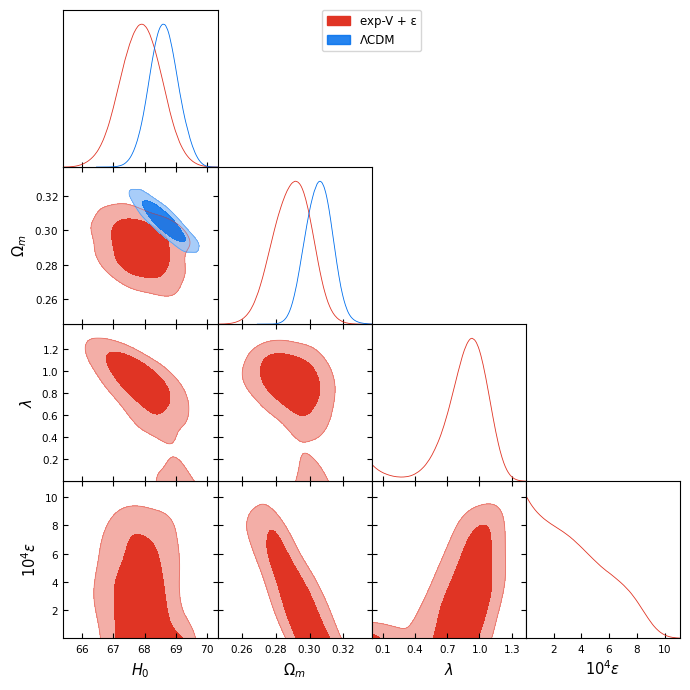
\includegraphics[width=0.75\textwidth]{triangle_planck_rd.png}
\caption{Posteriors of $H_0$, $\Omega_m$, $\lambda$ and $10^4\epsilon$ with the Planck $r_d$ prior, for $\Lambda$CDM (grey) and exp-$V$ + $\epsilon$ (blue).}\label{fig:triangle}
\end{figure}

Table~\ref{tab:fits} and Fig.~\ref{fig:triangle} show three things.
\begin{enumerate}
\item \emph{Quadratic gravity is not detected.} With $\Lambda$ the best fit is $\epsilon=0$, with $\epsilon<4.1\times10^{-4}$ at first order. This corresponds to $\aeff\lesssim8\times10^{48}\,{\rm m^2}$, or a scalaron heavier than $\sim20H_0$, valid only to order of magnitude (Secs.~\ref{sec:reduction} and~\ref{sec:validation}).
\item \emph{A rolling field is mildly preferred.} The improvement is $\Delta\chi^2=-4.94$, about $2.2\sigma$ for one parameter. It comes from BAO ($-2.3$) and supernovae ($-2.8$). AIC favours exp-$V$ weakly and BIC does not.
\item \emph{Once $V$ can roll, $\epsilon$ is no longer bounded by the data.} The exp-$V+\epsilon$ posterior reaches the prior edge, and $\Delta\chi^2$ relative to exp-$V$ is only $-0.3$.
\end{enumerate}
A two-sided profile illustrates the third point. With $\Lambda$ fixed, $\chi^2$ falls towards negative (unstable) $\epsilon$: it is lower by 1.8 at $\et=-6\times10^{-4}$. With $\lambda$ free, the minimum moves to $\et\approx+5\times10^{-4}$ and is flat to $\pm0.3$.

With $r_d$ free, the $\chi^2$ values, $\lambda$ and the $\epsilon$ bound ($<3.5\times10^{-4}$) are unchanged. Only the absolute scale loosens: $H_0=68.4^{+4.3}_{-4.2}$ for $\Lambda$CDM and $r_d=146.7^{+8.9}_{-7.9}$\,Mpc. Adding the other 17 measurements of the 32-point chronometer compilation~\cite{2201.07241}, as independent points without their systematic covariance, tightens this to $H_0=69.7^{+2.6}_{-2.3}$ and moves the $\epsilon$ bound to $3.8\times10^{-4}$. With the Planck $r_d$ prior the extra points change nothing: $H_0=68.66\pm0.48$ for $\Lambda$CDM, and $\lambda=0.78$ with $\Delta\chi^2=-5.0$ for exp-$V$.

\subsection{Free-form potential}
\begin{figure}[h]\centering
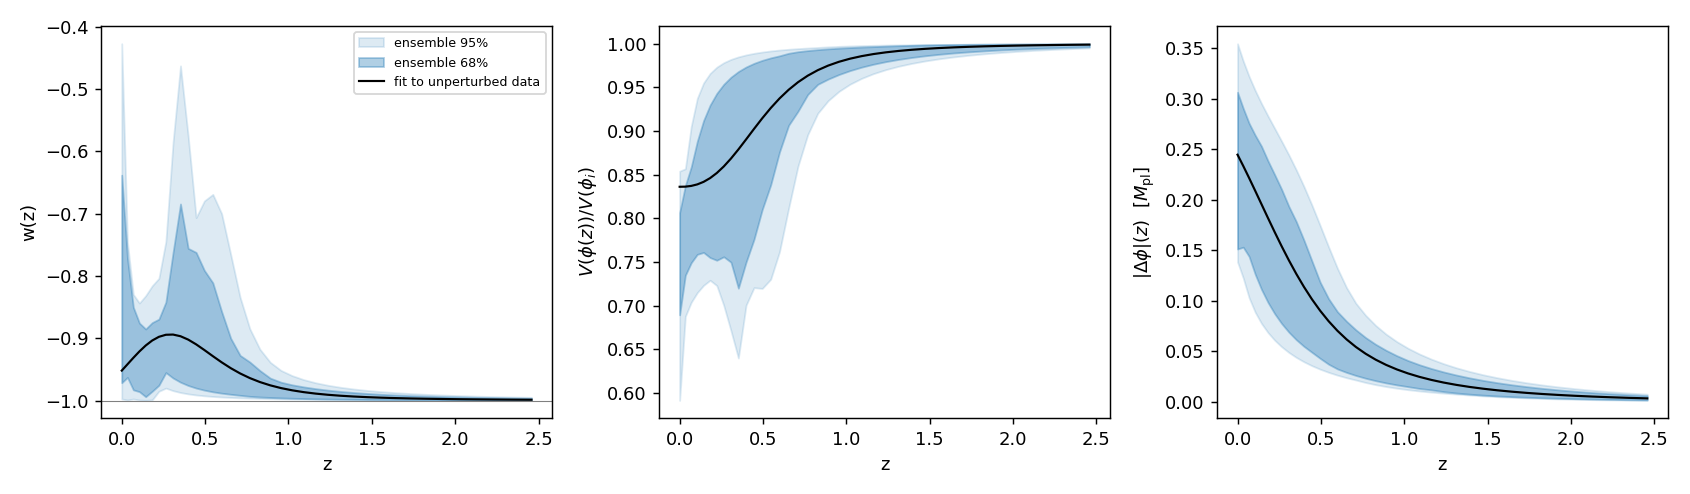
\includegraphics[width=\textwidth]{nn_planck.png}
\caption{Neural reconstruction on real data. Panels: $w(z)$, $V(\phi(z))/V(\phi_i)$ and $|\Delta\phi|(z)$. Shown are the fit to the unperturbed data (black) and the 68\% and 95\% ranges of the bootstrap members.}\label{fig:nn}
\end{figure}

The network (Fig.~\ref{fig:nn}) reaches $\chi^2=1400.77$ (CC/BAO/SN 6.46/8.28/1386.02). This is only 0.4 below the one-parameter exponential. On mocks the ensemble overstates the field excursion and the drop in $V$, so neither is by itself evidence of rolling (Sec.~\ref{sec:coverage}). The ensemble gives:
\begin{itemize}
\item $H_0=67.40^{+0.50}_{-0.47}$ and $\Omega_m=0.302^{+0.011}_{-0.012}$;
\item $w_0=-0.87^{+0.23}_{-0.10}$;
\item a field excursion $|\Delta\phi|=0.24^{+0.06}_{-0.09}\,\Mpl$, consistent with exp-$V$ ($0.25^{+0.06}_{-0.08}$).
\end{itemize}
Every member has $\dot\phi^2\ge0$ by construction. Many members show a bump in $w(z)$ near $z\approx0.3$. Sections~\ref{sec:fisher} and~\ref{sec:coverage} show that this feature is not data-driven. Adding $\epsilon$ to the network changes $\chi^2$ by $-0.17$.

\subsection{What the data measure about $V(\phi)$}\label{sec:fisher}
The fiducial is the exp-$V$ best fit ($\lambda=0.822$). Over the observed epoch the field moves by $0.254\,\Mpl$, so $\ln V$ changes by $0.21$.

\begin{table}[h]\centering\small
\caption{Fisher errors on the shape of $\ln V$ (top) and on $\et$ for increasing freedom in $V$ (bottom).}\label{tab:fisher}
\begin{tabular}{lccc}\toprule
$\ln V$ to order & $\sigma$(amplitude) & $\sigma$(slope) & $\sigma$(curvature)\\\midrule
linear & 0.045 & 0.175 & --\\
quadratic & 0.13 & 0.177 & 9.0\\
cubic & 0.28 & 0.182 & 9.2\\\bottomrule
\end{tabular}\\[8pt]
\begin{tabular}{lcc}\toprule
Freedom in $V$ & $\sigma(\et)$ & corr$(\et,\ln\omega_m)$\\\midrule
amplitude & $6.2\times10^{-4}$ & $-0.87$\\
+ slope & $9.0\times10^{-4}$ & $-0.94$\\
+ curvature & $1.65\times10^{-3}$ & $-0.98$\\
6 Legendre modes & $1.2\times10^{-2}$ & $-1.00$\\\bottomrule
\end{tabular}
\end{table}

The 6-mode Fisher matrix has eigen-errors 0.0044, 0.023, 0.051, 0.094, 0.19 and 1.3 (unit-norm combinations of Legendre coefficients). Five combinations are therefore limited to $\lesssim0.2$ in $\ln V$ across the traversed range. Whether that amounts to measuring a feature depends on how large a deformation a physical potential produces, and here the small field excursion decides. With the Legendre polynomials on $[0,\Delta\phi]$ and $\Delta\phi=0.254\,\Mpl$:
\begin{itemize}
\item a slope $|V'/V|=1\,\Mpl^{-1}$ gives a $P_1$ coefficient $\Delta\phi/2\approx0.13$, against a Fisher error of 0.022;
\item a curvature $|V''/V|=1\,\Mpl^{-2}$ gives a $P_2$ coefficient $\Delta\phi^2/12\approx0.005$, against a Fisher error of 0.048.
\end{itemize}
By this criterion the data measure the height and the slope. The slope error is stable at $0.18\,\Mpl^{-1}$ as freedom is added. A curvature would have to exceed $|V''/V|\approx9\,\Mpl^{-2}$ to be seen at $1\sigma$, an order of magnitude beyond the values of order unity typical of thawing models. Any feature beyond a straight line in a reconstructed $\ln V(\phi)$ therefore comes from the prior, the kernel or the initialisation.

Two remarks on the slope. First, $\sigma=0.18$ is a local error at $\lambda=0.82$, while the preference for a non-zero slope is only $\Delta\chi^2=-4.9$, about $2.2\sigma$. The two agree because near $\lambda=0$ the observables respond to $\lambda^2$, since $1+w\propto\lambda^2$ at leading order~\cite{2608.13488}. The significance of $\lambda\neq0$ is then about $\lambda/(2\sigma_\lambda)\approx2.3$.
Second, Park et al.\ find four to five constrained quintessence parameters~\cite{2101.04666}. Their count is for the EFT function $\Delta\Lambda(a)$ on a spline in time, measured against a correlation prior, with CMB, CMB-lensing, BAO, galaxy and supernova data. Ours is a local Fisher count for $\ln V(\phi)$ with background data only. The two counts answer different questions and do not conflict.

Conversely, the bound on $\epsilon$ weakens twenty-fold as $V$ is freed and becomes fully degenerate with $\omega_m$. Quadratic-gravity bounds quoted with $\Lambda$ fixed are conditional on $\Lambda$.

\subsection{Calibration of the ensemble on mocks}\label{sec:coverage}
\paragraph{Single closure test.} We generated mock data from $V\propto e^{-\phi}$ ($H_0=63.76$). The network's 95\% band contains the true $V$ at all redshifts, but its 68\% band does so at only 42\% of them. It also overestimates the field excursion: 0.48 for the member fitted to the mock, against a true 0.277.
An exponential fit to the same mock is displaced in the same direction ($\Delta\chi^2=3.9$ from truth). Part of the offset is therefore the noise realisation, and the rest is the network fitting noise in unconstrained directions (Fig.~\ref{fig:closure}).

\begin{figure}[h]\centering
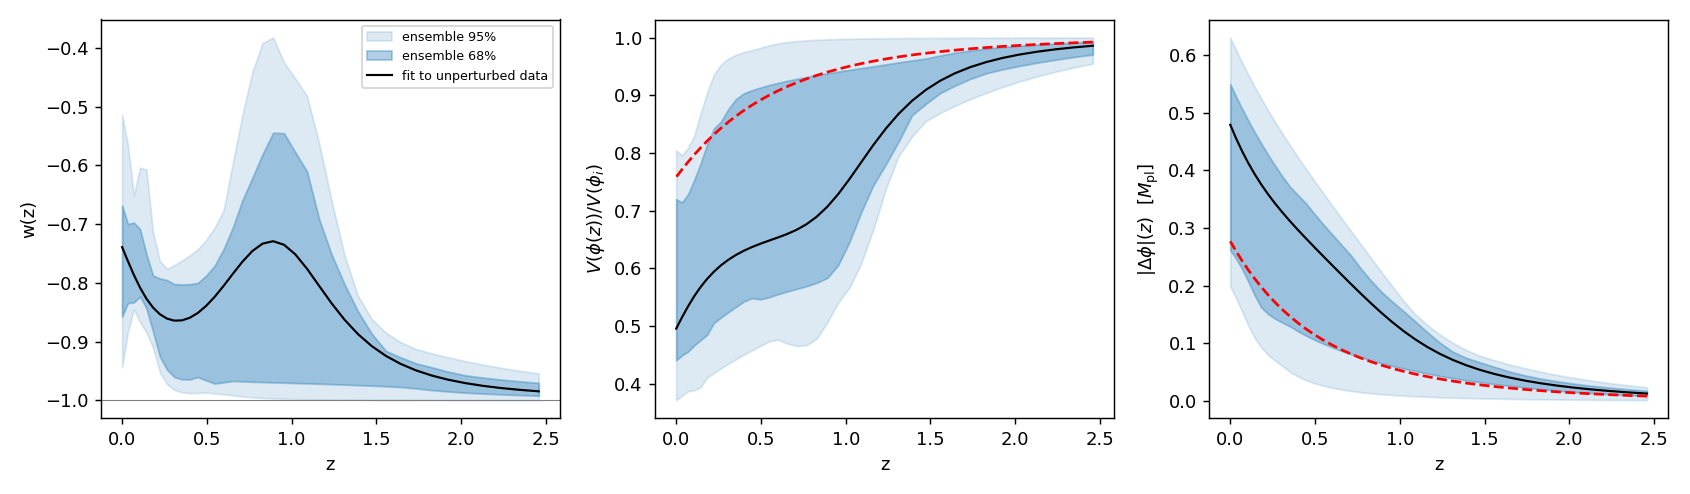
\includegraphics[width=\textwidth]{nn_planck_mock.png}
\caption{Closure test on one mock generated from $V\propto e^{-\phi}$. Panels as in Fig.~\ref{fig:nn}; the truth is shown dashed in red.}\label{fig:closure}
\end{figure}

\paragraph{50-mock coverage.} One realisation cannot establish calibration. We therefore drew 50 mock skies from the real covariances around the exp-$V$ best fit, fluctuating the $r_d$ measurement as well. The truth is $H_0=67.77$, $\Omega_m=0.303$, $w_0=-0.896$, $|\Delta\phi|=0.254$.
Each sky was analysed three ways:
\begin{enumerate}
\item the neural ensemble exactly as above;
\item emcee with $\ln V=\ln V_0-\lambda\phi+c_2\phi^2/2$, i.e.\ the two shape modes of Table~\ref{tab:fisher} ($c_2\in[-30,30]$);
\item emcee with the true exponential family, as a well-specified reference.
\end{enumerate}

\begin{table}[h]\centering\small
\caption{Coverage on 50 mocks: percentage whose central 68\% / 95\% interval contains the truth, and mean bias of the medians in units of the mean $1\sigma$ width. Binomial $1\sigma$: $\pm6.6\%$ / $\pm3.1\%$. For the 23-member ensemble the effective levels are 67\% / 92\% ($\pm3.8\%$; Sec.~\ref{sec:method}).}\label{tab:coverage}
\begin{tabular}{lcccccc}\toprule
& \multicolumn{2}{c}{Neural ensemble} & \multicolumn{2}{c}{emcee, slope + curvature} & \multicolumn{2}{c}{emcee, exponential}\\
Quantity & 68 / 95 & bias & 68 / 95 & bias & 68 / 95 & bias\\\midrule
$H_0$ & 54 / 88 & $-0.15$ & 60 / 94 & $+0.44$ & 58 / 88 & $\le0.08$\\
$\Omega_m$ & 56 / 96 & $-0.25$ & 62 / 100 & $-0.26$ & 64 / 96 & $\le0.08$\\
$w_0$ & 82 / 98 & $+0.09$ & 64 / 92 & $-0.65$ & 80 / 94 & $\le0.08$\\
$|\Delta\phi|$ & 66 / 94 & $-0.14$ & 82 / 96 & $-0.20$ & 80 / 94 & $\le0.08$\\
$V_0/V_i$ & 78 / 100 & $-0.49$ & 80 / 96 & $-0.01$ & 80 / 94 & $\le0.08$\\
\bottomrule\end{tabular}
\end{table}

\begin{figure}[h]\centering
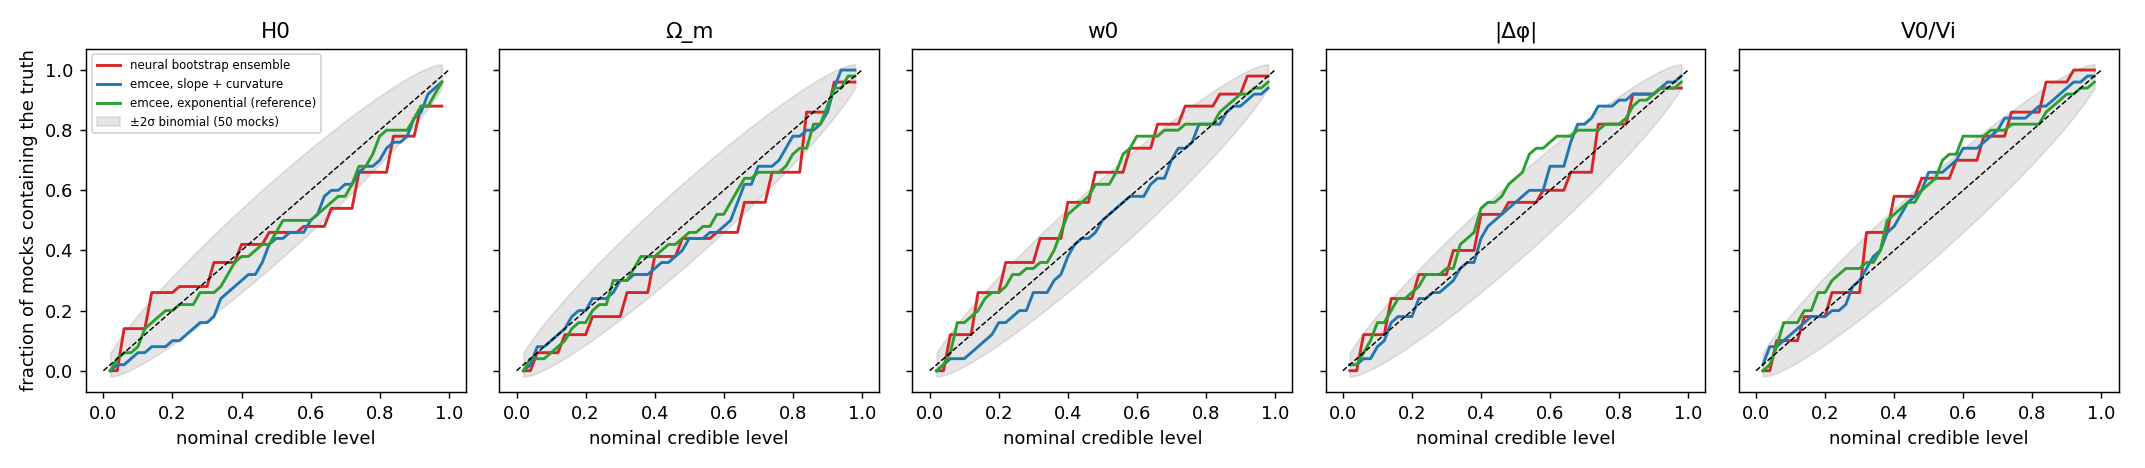
\includegraphics[width=\textwidth]{coverage.png}
\caption{Empirical coverage against nominal credible level for the three methods (50 mocks). The grey band is the $\pm2\sigma$ binomial range.}\label{fig:coverage}
\end{figure}

Table~\ref{tab:coverage} and Fig.~\ref{fig:coverage} lead to four conclusions.
\begin{itemize}
\item \emph{The ensemble is about as well calibrated as a sampled posterior.} Against its effective levels (67\% / 92\%), its coverage at this truth lies within about $2\sigma$ everywhere. It is conservative at the outer level for $\Omega_m$, $w_0$ and $V_0/V_i$, and at 68\% for $w_0$.
\item \emph{The low $H_0$ coverage of the ensemble is not reproduced on independent noise.} At 68\% all three methods cover $H_0$ in only 54--60\% of these 50 skies. We therefore drew 100 new skies with an independent noise seed and reran the ensemble and the exponential reference. On them the ensemble is nominal for every quantity: 65--75\% at 68\% and 88--98\% at 95\%, with $H_0$ at 67\% / 91\% and no bias, although its $H_0$ half-width is still about 10\% below the scatter of the medians. Only the $V_0/V_i$ bias recurs ($-0.40\sigma$). The exponential reference still under-covers $H_0$ (60\% / 91\%; 59\% over all 150 skies, $2.3\sigma$ low). On the new skies its medians are also biased towards less roll ($+0.35\pm0.11\sigma$ in $H_0$, $-0.44\pm0.10\sigma$ in $w_0$), while on the first 50 skies, with identical settings, they were not ($-0.01\pm0.13\sigma$ in $w_0$). The two seeds disagree at $2.7\sigma$; we have no explanation and report both.
\item \emph{The network has a residual bias.} $V_0/V_i$ is pulled low by $0.49\sigma$, i.e.\ the network prefers slightly more roll than the truth, consistent with the closure test. The bias doubles when the field barely rolls (below).
\item \emph{Curvature freedom costs a bias in $w_0$.} The slope + curvature chains trade curvature against slope and are biased in $w_0$ by $-0.65\sigma$. Near $\lambda=0$ this becomes a failure (below).
\end{itemize}
The slope + curvature chains ran 12\,000 steps, reaching 41 autocorrelation times at the median and 29 at the minimum. An earlier 4000-step run (23 autocorrelation times) gave coverages within 8 points of these.

\paragraph{A barely rolling truth.} We repeated the test with $\lambda=0.30$: $H_0=68.53$, $\Omega_m=0.3045$, $w_0=-0.986$, $|\Delta\phi|=0.088$, $V_0/V_i=0.974$. The mocks reuse the noise draws of the first truth. Differences between Tables~\ref{tab:coverage} and~\ref{tab:coverageB} are therefore caused by the truth. Features common to both, such as the low $H_0$ and $\Omega_m$ coverage at 68\% (52--62\% here), are not independent confirmations. The slope + curvature chains reached 47 autocorrelation times at the median (29 at the minimum), the exponential chains 170 (137).

\begin{table}[h]\centering\small
\caption{As Table~\ref{tab:coverage}, for the barely rolling truth ($\lambda=0.30$) and the same noise draws.}\label{tab:coverageB}
\begin{tabular}{lcccccc}\toprule
& \multicolumn{2}{c}{Neural ensemble} & \multicolumn{2}{c}{emcee, slope + curvature} & \multicolumn{2}{c}{emcee, exponential}\\
Quantity & 68 / 95 & bias & 68 / 95 & bias & 68 / 95 & bias\\\midrule
$H_0$ & 56 / 92 & $-0.32$ & 62 / 96 & $+0.18$ & 56 / 96 & $-0.21$\\
$\Omega_m$ & 52 / 90 & $-0.42$ & 56 / 96 & $-0.23$ & 60 / 98 & $-0.08$\\
$w_0$ & 88 / 98 & $+0.30$ & 32 / 96 & $-1.21$ & 94 / 98 & $+0.49$\\
$|\Delta\phi|$ & 80 / 98 & $+0.66$ & 100 / 100 & $+0.03$ & 94 / 98 & $+0.46$\\
$V_0/V_i$ & 72 / 98 & $-1.00$ & 96 / 100 & $-0.43$ & 94 / 98 & $-0.49$\\
\bottomrule\end{tabular}
\end{table}

\begin{figure}[h]\centering
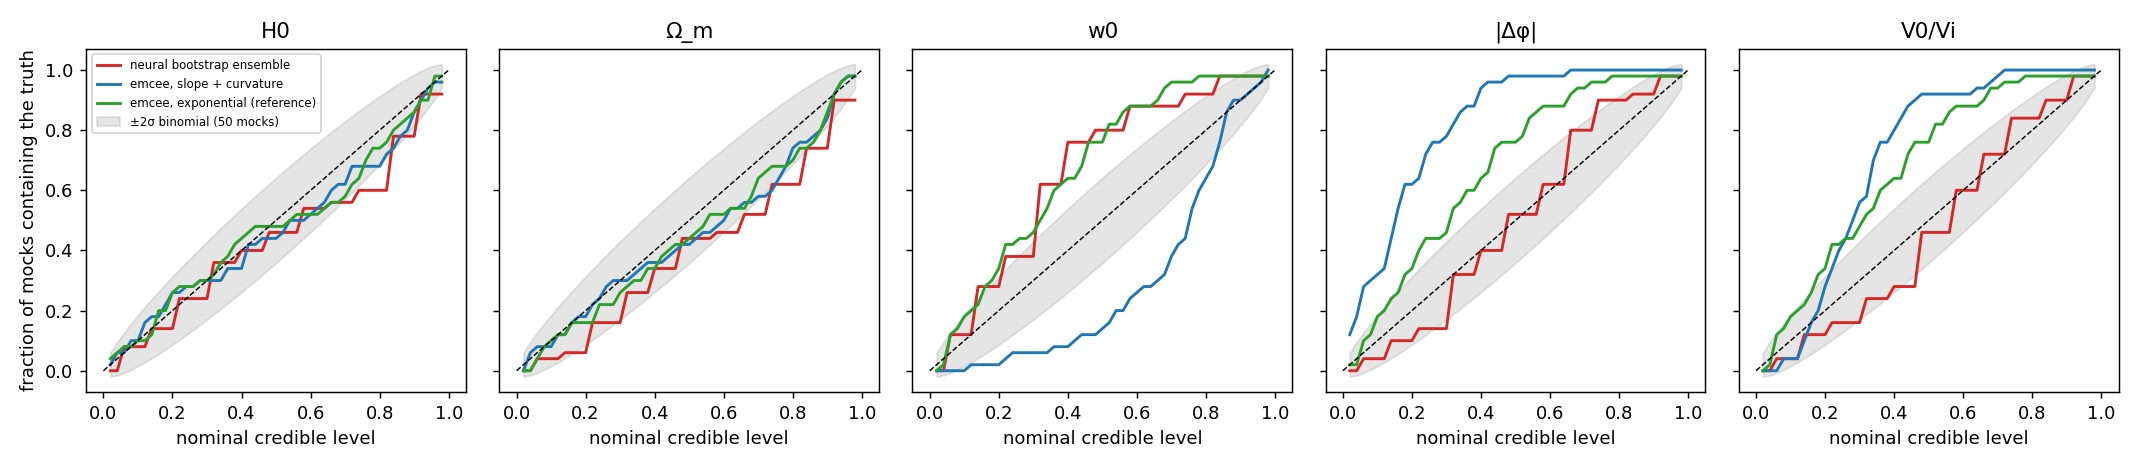
\includegraphics[width=\textwidth]{coverage_B.png}
\caption{As Fig.~\ref{fig:coverage}, for the barely rolling truth ($\lambda=0.30$).}\label{fig:coverageB}
\end{figure}

Table~\ref{tab:coverageB} and Fig.~\ref{fig:coverageB} add three conclusions.
\begin{itemize}
\item \emph{Near $\lambda=0$ the intervals on the shape of $V$ are conservative.} At 68\% the MCMC intervals contain the true $|\Delta\phi|$ and $V_0/V_i$ in 94--100\% of skies, with half-widths up to twice the scatter of the medians, as expected for posteriors cut at $\lambda=0$ when the data constrain only $\lambda^2$. The ensemble is closer to nominal (72--88\% for $w_0$, $|\Delta\phi|$ and $V_0/V_i$).
\item \emph{The medians overstate the roll.} The ensemble's median $V_0/V_i$ averages $0.856$ against a true $0.974$, i.e.\ a 14\% drop in $V$ where the truth has 2.6\%, and its median $|\Delta\phi|$ averages $0.157$ against $0.088$. In units of the interval width the $V_0/V_i$ bias is $-1.00\sigma$, twice that at the first truth. The exponential reference is biased the same way ($-0.49\sigma$ and $+0.46\sigma$), but its absolute shift in $V_0/V_i$ (0.028) is four times smaller. Ref.~\cite{2505.10662} report the same effect on $\Lambda$CDM mocks, which return a non-zero linear term in $V$; their parametrisation and truth differ from ours, so the comparison is qualitative.
\item \emph{Slope + curvature fails for $w_0$.} Its 68\% interval contains the true $w_0$ in only 32\% of skies, $5.5$ binomial $\sigma$ below nominal. The median averages $-0.997$ and the half-width ($0.009$) is a third of the exponential chains', while the 95\% interval still covers (96\%). The posterior is piled against $w=-1$. Rerunning three of the failing chains with their samples kept shows why; the reruns reproduce the failure, with the true $w_0$ at the 88th--90th percentile. In each, 78--83\% of the samples have $w_0<-0.995$, and 97--98\% of those have $c_2>0$, typically $c_2\approx18$ with a steep initial slope $\lambda\approx1.1$. Then $\ln V$ has a minimum at $\phi=\lambda/c_2\approx0.06$, and the field sits there today. The best fits inside and outside this region differ by $|\Delta\chi^2|<0.7$, so the data do not prefer halted fields. The pile is prior volume: the flat prior $c_2\le30$ admits a long family of halted potentials. Near $\lambda=0$ the $w_0$ of this model therefore reflects the prior on $c_2$, which the data do not measure (Sec.~\ref{sec:fisher}).
\end{itemize}

The same mocks test whether a barely rolling universe could produce the real-data preference for rolling. In one of the 50 skies the exponential fit reaches the real-data median $w_0=-0.90$ (Table~\ref{tab:fits}), and in one its median $|\Delta\phi|$ reaches the real-data median $0.25$. For the ensemble, two skies reach its real-data median $w_0=-0.87$, but six reach its real-data median $|\Delta\phi|=0.24$. A barely rolling universe thus reproduces the fitted $w_0$ in at most 2 of 50 skies but the network's field excursion in 6 of 50 (12\%), so the excursion in Fig.~\ref{fig:nn} is at most weak evidence of rolling.

\subsection{The Hubble constant}
\begin{table}[h]\centering\small
\caption{$H_0$ with the Planck $r_d$ prior, and tension with SH0ES ($73.04\pm1.04$~\cite{2112.04510}) and Planck $\Lambda$CDM ($67.36\pm0.54$~\cite{1807.06209}).}\label{tab:h0}
\begin{tabular}{lccc}\toprule
Model & $H_0$ & vs SH0ES & vs Planck\\\midrule
$\Lambda$CDM & $68.61\pm0.45$ & $3.9\sigma$ & $1.8\sigma$\\
$\Lambda$CDM$+\epsilon$ & $68.70^{+0.53}_{-0.48}$ & $3.7\sigma$ & $1.8\sigma$\\
exp-$V$ & $67.81^{+0.68}_{-0.57}$ & $4.3\sigma$ & $0.5\sigma$\\
exp-$V+\epsilon$ & $67.89\pm0.66$ & $4.2\sigma$ & $0.6\sigma$\\
neural $V$ (ensemble) & $67.40^{+0.50}_{-0.47}$ & $4.9\sigma$ & $0.1\sigma$\\\bottomrule
\end{tabular}
\end{table}

No model eases the tension, and the scalar field makes it slightly worse (Table~\ref{tab:h0}). Two mechanisms are at work:
\begin{itemize}
\item A thawing field lowers the dark-energy density today relative to the past. At fixed $r_d$, $H_0$ therefore decreases.
\item The $\epsilon$ term adds expansion at $z\gtrsim1$, not at $z=0$, so it cannot raise $H_0$ either.
\end{itemize}
Raising $H_0$ with the inverse distance ladder requires a smaller sound horizon. This action cannot provide one, because its correction vanishes in the radiation era. With $r_d$ free, the chronometers alone are too imprecise to bear on the tension: even the 32-point compilation gives $H_0=69.7^{+2.6}_{-2.3}$, $1.2\sigma$ from SH0ES and $1.0\sigma$ from Planck.

%=====================================================================
\section{Discussion and limitations}\label{sec:discussion}
%=====================================================================
\paragraph{What the method adds.} The gain is not raw speed. For a single parameter set, an adaptive SciPy solver (10\,ms) beats our RK4 (78\,ms); RK4 wins only when batched. The gain is exact derivatives:
\begin{itemize}
\item The gradient of $\chi^2$ with respect to all 323 parameters costs 0.4\,s, against about 110\,s for finite differences (extrapolated).
\item A function-space Jacobian, which is what makes Sec.~\ref{sec:fisher} possible, costs 9 forward-mode passes.
\end{itemize}
MCMC remains necessary where posteriors are non-Gaussian: Fisher underestimates $\sigma(\lambda)$ by 23\%.

\paragraph{Limitations.}
\begin{itemize}
\item \emph{The order reduction limits the $\epsilon$ bound to order of magnitude} (Secs.~\ref{sec:reduction} and~\ref{sec:validation}). The reduced series is asymptotic, so going to higher order cannot sharpen it. A sharper bound needs the full equation and a physical prescription for the scalaron initial data.
\item \emph{Background only.} We include no growth, lensing or CMB. The spin-2 ghost and local bounds lie outside the analysis.
\item \emph{The model is defined for $z\le4$,} with $r_d$ external. $H_0$ values with the Planck prior assume standard physics at higher redshift.
\item \emph{Calibration and mode counting have limited scope.} Calibration is tested at two truths ($\lambda=0.82$ and $0.30$) on the same 50 noise draws, plus 100 independent draws at the first, and not for strongly curved potentials. Mode counting is done at one fiducial ($\lambda=0.82$); near $\lambda=0$ the field does not move and no shape information is measurable.
\item \emph{Data choices.} We use 15 rather than 32 chronometer points, Pantheon+ only, 1580 rather than 1590 SNe, and massless neutrinos. DES-SN5YR and Union3 favour dynamical dark energy more strongly than Pantheon+.
\end{itemize}

%=====================================================================
\section{Conclusions}
%=====================================================================
A free-form version of direct reconstruction, with a neural potential inside the exact field equations, gives reconstructions that are solutions of the theory. It also gives the exact Jacobians needed to ask what the data measure. For chronometers, DESI DR2 BAO and Pantheon+, the answer is the height and slope of $\ln V$, a limit set by the small field excursion:
\begin{itemize}
\item a 321-parameter network fits only 0.4 better in $\chi^2$ than an exponential;
\item the curvature of $\ln V$ is unconstrained;
\item features in reconstructed $w(z)$ beyond a monotonic thaw are not data-driven.
\end{itemize}
On mocks at two truths the bootstrap ensemble's intervals are about as well calibrated as MCMC posteriors, but its median overstates the roll by $0.5$--$1\sigma$, most when the field barely rolls.

A quadratic-gravity correction, of which only $\alpha+\beta/3$ is observable, is not detected. Its bound is conditional on $\Lambda$ and degenerates with $\omega_m$ when $V$ is free. At the bound, the order-reduced description is accurate only to order of magnitude. None of the models eases the $H_0$ tension.

\paragraph{Code and data availability.} All code, data-loading scripts and result summaries are available at \url{https://github.com/NiksheyYadav/dark-energy-potential}. \todo{make the repository public and tag the submitted version.}

\paragraph{Use of AI tools.} Claude (Anthropic), a large language model, assisted with writing and debugging the analysis code, running and summarising the numerical experiments, checking references and drafting the text. The author directed the study, checked the derivations, code and results, and takes full responsibility for the content. \todo{confirm this statement matches your contribution, and check your university's and the journal's AI policy.}

\paragraph{Acknowledgments.} \todo{supervisor, institution, funding.}

\bibliographystyle{unsrtnat}
\bibliography{refs}

\appendix
%=====================================================================
\section{Variation of the quadratic terms}\label{app:variation}
%=====================================================================
Using $\delta\sqrt{-g}=-\tfrac12\sqrt{-g}\,g_{\mu\nu}\delta g^{\mu\nu}$, $\delta R=R_{\mu\nu}\delta g^{\mu\nu}+(g_{\mu\nu}\Box-\nabla_\mu\nabla_\nu)\delta g^{\mu\nu}$, integration by parts and $\nabla^\mu R_{\mu\nu}=\tfrac12\nabla_\nu R$:
\begin{align}
E^{(1)}_{\mu\nu}&=2RR_{\mu\nu}-\tfrac12g_{\mu\nu}R^2+2(g_{\mu\nu}\Box-\nabla_\mu\nabla_\nu)R,\\
E^{(2)}_{\mu\nu}&=-\tfrac12g_{\mu\nu}R_{\alpha\beta}R^{\alpha\beta}+2R_{\mu\alpha\nu\beta}R^{\alpha\beta}+\Box R_{\mu\nu}+\tfrac12g_{\mu\nu}\Box R-\nabla_\mu\nabla_\nu R,\\
T^{(\phi)}_{\mu\nu}&=\partial_\mu\phi\,\partial_\nu\phi-g_{\mu\nu}\left[\tfrac12(\partial\phi)^2+V\right].
\end{align}
On flat FLRW with lapse $N(t)$, varying the minisuperspace action with respect to $N$ gives Eq.~\eqref{eq:friedmann}. The $R^2$ term contributes $36\,(6H^2\dot H+2H\ddot H-\dot H^2)$ and the $R_{\mu\nu}R^{\mu\nu}$ term $12\,(\ldots)$ with the same bracket. This was checked with SymPy (\texttt{symbolic\_check.py}).

\end{document}
